\chapter{Results}

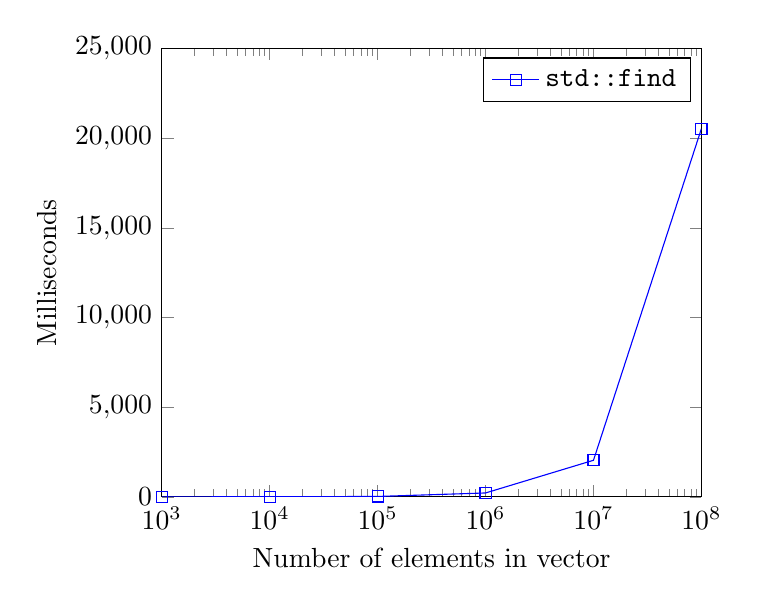
\begin{tikzpicture}
\begin{axis}[
    xmin=10^3, xmax=10^8,
    ymin=0, ymax=25000,
    xmode=log,
    ymode=linear,
    yticklabel style={
        /pgf/number format/fixed,
        /pgf/number format/precision=4
    },
    scaled y ticks=false,
    ylabel=Milliseconds,
    xlabel=Number of elements in vector
]

\addplot[
    color=blue,
    mark=square,
    ]
    coordinates {
    (10^3,0.207)(10^4,2.025)(10^5,20.032)(10^6,215.423)(10^7,2038.319)(10^8,20531.186)
    };
\legend{\texttt{std::find}}
\end{axis}
\end{tikzpicture}

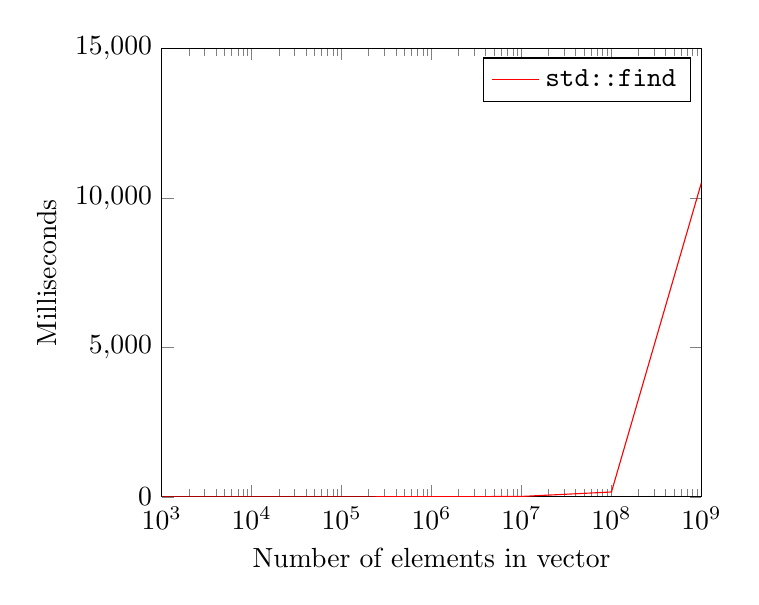
\begin{tikzpicture}
\begin{axis}[
    xmin=10^3, xmax=10^9,
    ymin=0, ymax=15000,
    xmode=log,
    ymode=linear,
    yticklabel style={
        /pgf/number format/fixed,
        /pgf/number format/precision=4
    },
    scaled y ticks=false,
    ylabel=Milliseconds,
    xlabel=Number of elements in vector
]

\addplot[
    color=red,
    mark=circle,
    ]
    coordinates {
    (10^3,0.001)(10^4,0.012)(10^5,0.115)(10^6,1.236)(10^7,12.650)(10^8,161.944)(10^9,10509.018)
    };
\legend{\texttt{std::find}}

\end{axis}
\end{tikzpicture}
